\section{Background and Observations}

In this section, we first study the typical shuffle characteristics (\ref{shuffle pattern}), and then spot the opportunities to achieve shuffle optimization (\ref{observation}).
\subsection{Characteristic of Shuffle} \label{shuffle pattern}

In large scale data parallel computing, shuffle is designed to achieve an all-to-all data transfer among nodes. 
For a clear illustration, we use \textit{map tasks} to define the tasks that produce shuffle data and use \textit{reduce tasks} to define the tasks that consume shuffle data.
% Note that one task may have both shuffle data generation and consumption in modern DAG framework. These tasks contain characteristic of both map task and reduce task. But these tasks won't change the behavior of shuffle. To avoid ambiguity, in the following paper, we will only use term of map task to represent those who produce shuffle output, and reduce task to represent those who consume shuffle output.
% \begin{figure}
% 	\centering
% 	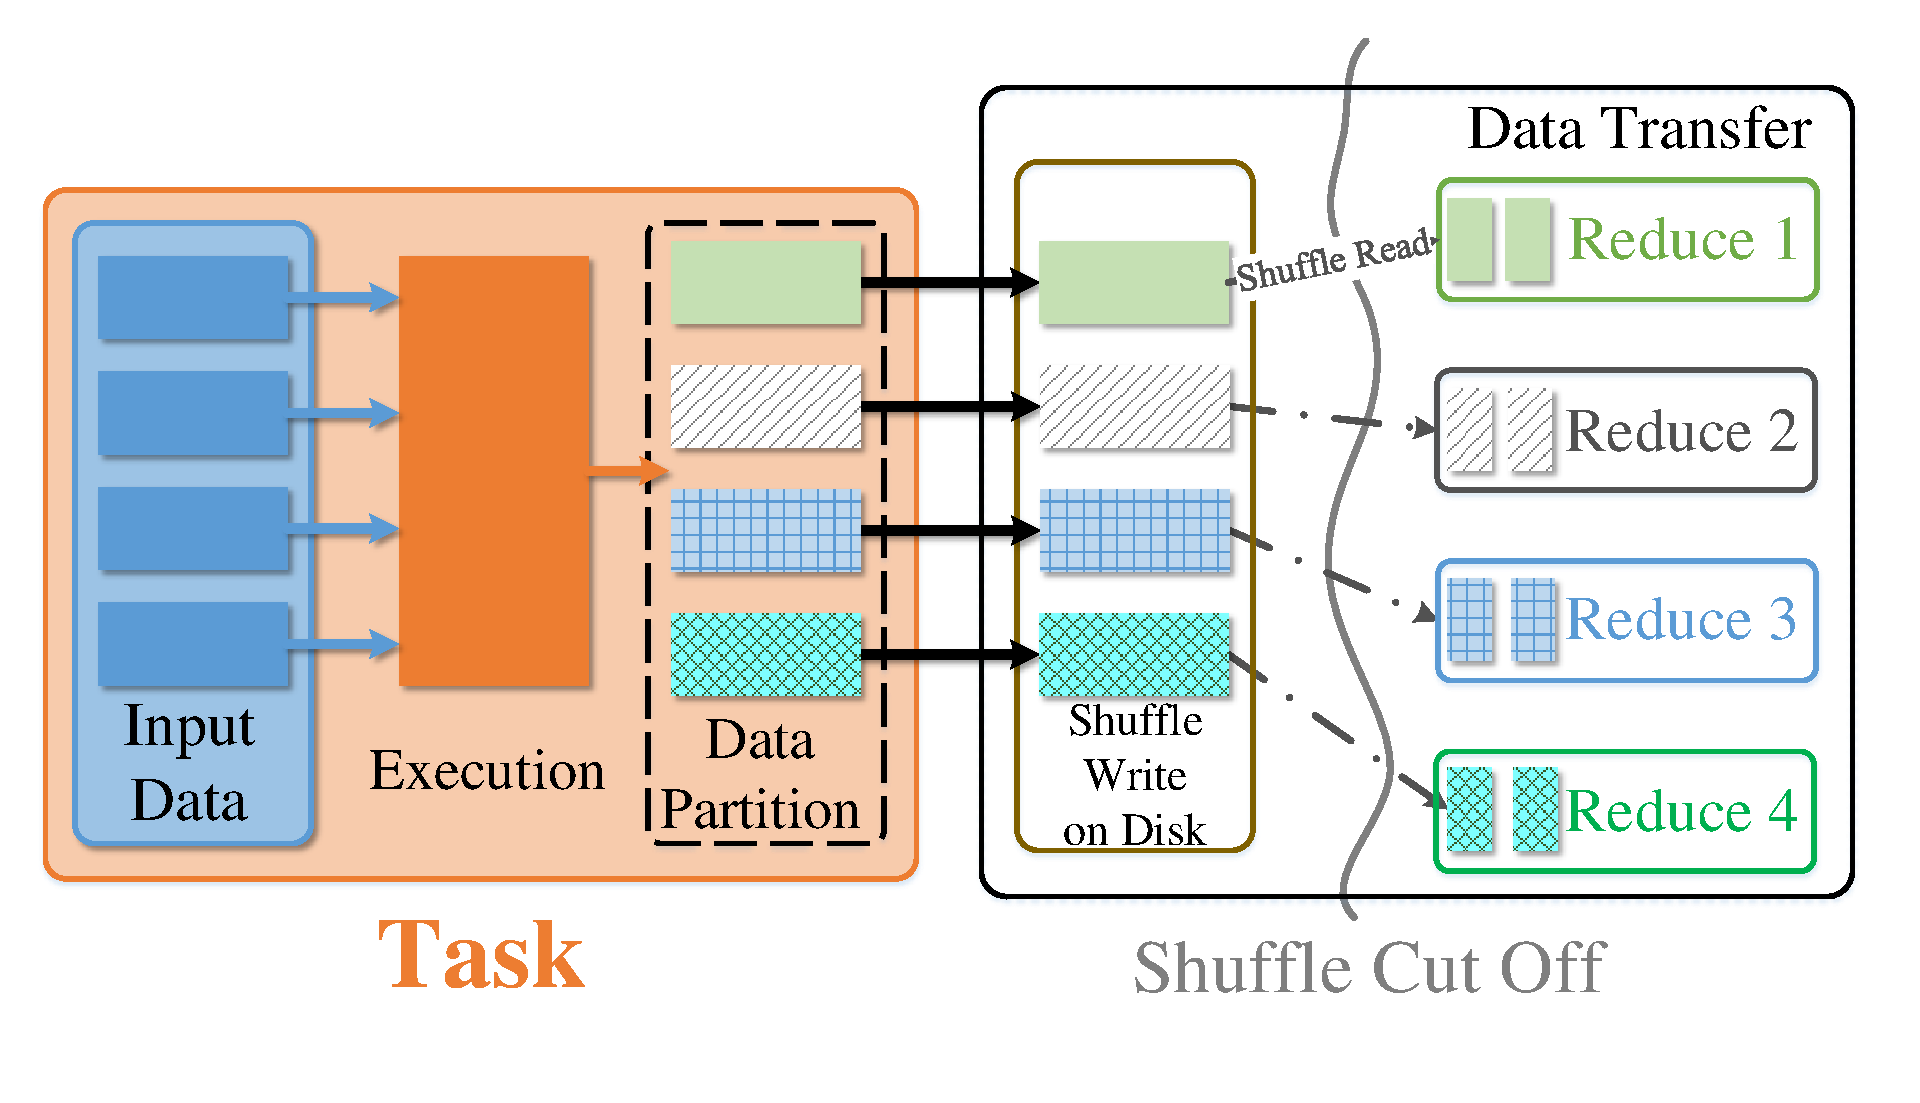
\includegraphics[width=\linewidth]{fig/shuffle_process}
% 	\caption{Shuffle Overview}
% 	\label{fig:shuffle_process}
% \end{figure}

\textbf{Overview of shuffle process}. 
Each map task partitions the result data (key, value pair) into several buckets according to the partition function (e.g., hash). 
The total number of buckets equals the number of reduce tasks in the successive step.
% shuffle data is produced by \textit{data partition}. For \textit{data partition}, 
The shuffle process can be further split into two parts: \textit{shuffle write} and \textit{shuffle read}. 
Shuffle write starts at the end of a map task and writes the partitioned map output data to local persistent storage. 
Shuffle read starts at the beginning of a reduce task and fetches the partitioned data from remote as its input. 

%In short, shuffle is loosely coupled with application context and it's I/O intensive.
\textbf{Impact of shuffle process}. Shuffle is I/O intensive, which might introduce a significant latency to the application. 
Reports show that $60\%$ of MapReduce jobs at Yahoo! and $20\%$ at Facebook are shuffle-heavy workloads \cite{shufflewatcher}. 
For those shuffle-heavy jobs, the shuffle latency may even dominate Job Completion Time (JCT).
For instance, a MapReduce trace analysis from Facebook shows that shuffle accounts for $33\%$ JCT on average, up to $70\%$ in shuffle-heavy jobs \cite{managing}.
% Besides, the completion time of shuffle correlates with the performance of storage devices, network and even applications.
% This variation may bring a huge challenge for operators to find the correct configuration of the DAG framework.

\subsection{Observations} \label{observation}
% Of course, shuffle is unavoidable in a DAG computing process. 
Can we mitigate or even remove the overhead of shuffle? 
To find the answers, we ran some typical Spark applications on a 5-node \texttt{m4.xlarge} EC2 cluster and analyzed the design and implementation of shuffle in some DAG frameworks.
Here we present the hardware utilization trace of one node running Spark's \textit{GroupByTest} in Figure \ref{fig:util} as an example. 
This job has 2 rounds of tasks for each node.
The \textit{Map Execution} is marked from the launch time of the first map task to the execution end time of the last one. 
The \textit{Shuffle Write} is marked from the beginning of the first shuffle write in the map stage. 
The \textit{Shuffle Read and Reduce Execution} is marked from the launch time of the first reduce task.
% Figure \ref{fig:util} reveals the performance information of two stages that are connected by shuffle. By analyzing the trace with Spark source code \cite{sparksource}, we propose the following observations.
% \begin{figure*}
% 	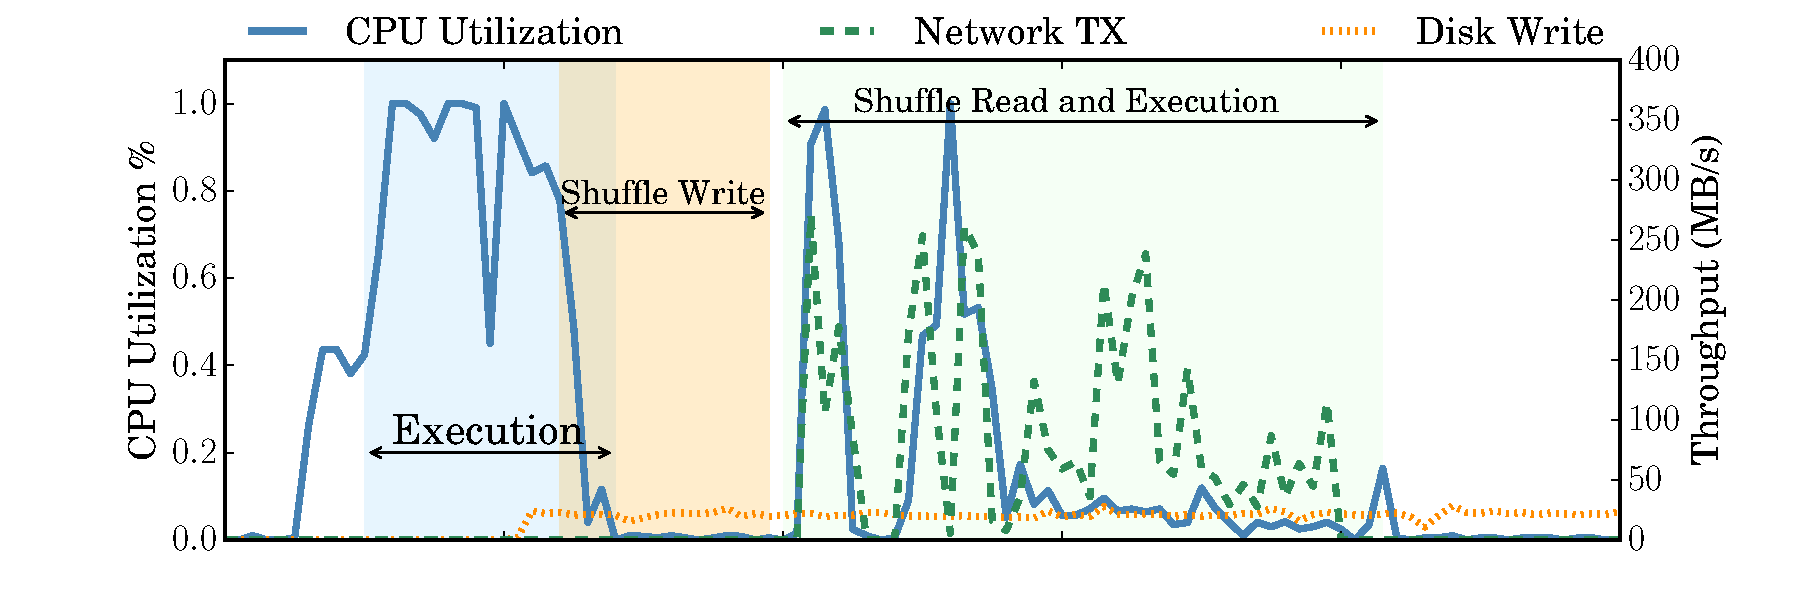
\includegraphics[width=\textwidth]{fig/util}
% 	\caption{CPU utiliazation and I/O throughput of a node during a Spark single shuffle application}
% 	\label{fig:util}
% \end{figure*}
\subsubsection{Coarse Granularity Resource Allocation}
When a slot is assigned to a task, it will not be released until the task completes (i.e., the end of shuffle write in Figure \ref{fig:util}). 
On the reduce side, the network transfer of shuffle data introduces an explicit I/O delay during shuffle read (i.e., the beginning of shuffle read and execution in Figure \ref{fig:util}). 
Meanwhile, both shuffle write and shuffle read occupy the slot without significantly involving CPU as presented in Figure \ref{fig:util}. 
The current coarse slot-task mapping results in an imbalance between task's resource demand and slot allocation thus decreasing the resource utilization. 
Unfortunately this defect exists not only in Spark \cite{apachespark} but also Hadoop MapReduce and Apache Tez \cite{tez}. 
A finer granularity resource allocation scheme should be provided to reduce these delays. 

\subsubsection{Synchronized Shuffle Read}
Almost all reduce tasks start shuffle read simultaneously. 
The synchronized shuffle read requests cause a burst of network traffic. 
As shown in Figure \ref{fig:util}, 
the data transfer causes a high demand of network bandwidth, which may result in network congestion and further slow down the network transfer.
It also happens in other frameworks that follow Bulk Synchronous Parallel (BSP) paradigm, such as Hadoop MapReduce, Dryad \cite{dryad}, etc.
% The previous work \cite{coflow, managing} also proves that the network transfer can introduce significant overhead in DAG computing.
\begin{figure*}
	\centering
	\begin{subfigure}[b]{0.47\linewidth}
		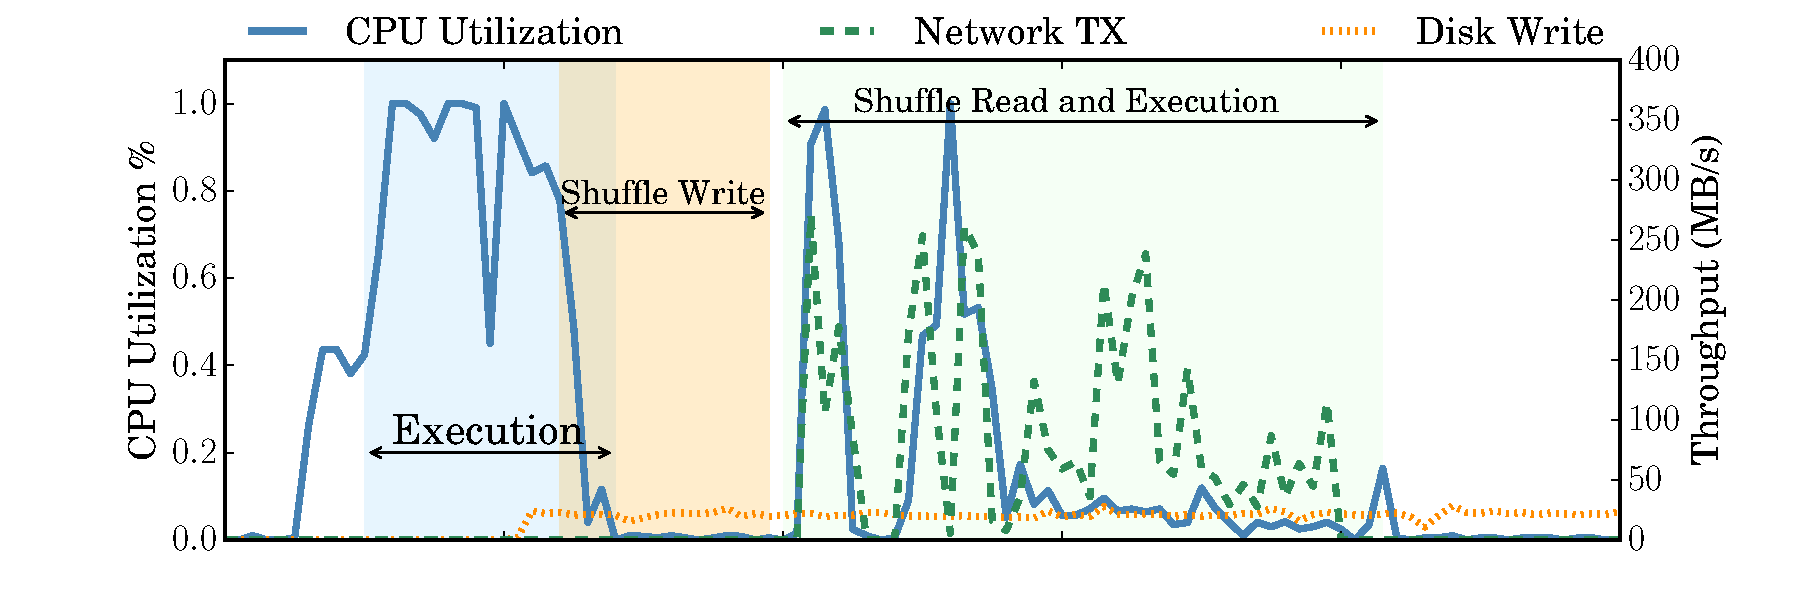
\includegraphics[width=\linewidth]{fig/util}
		\caption{Original Spark}
		\label{fig:util}
	\end{subfigure}
	\begin{subfigure}[b]{0.47\linewidth}
		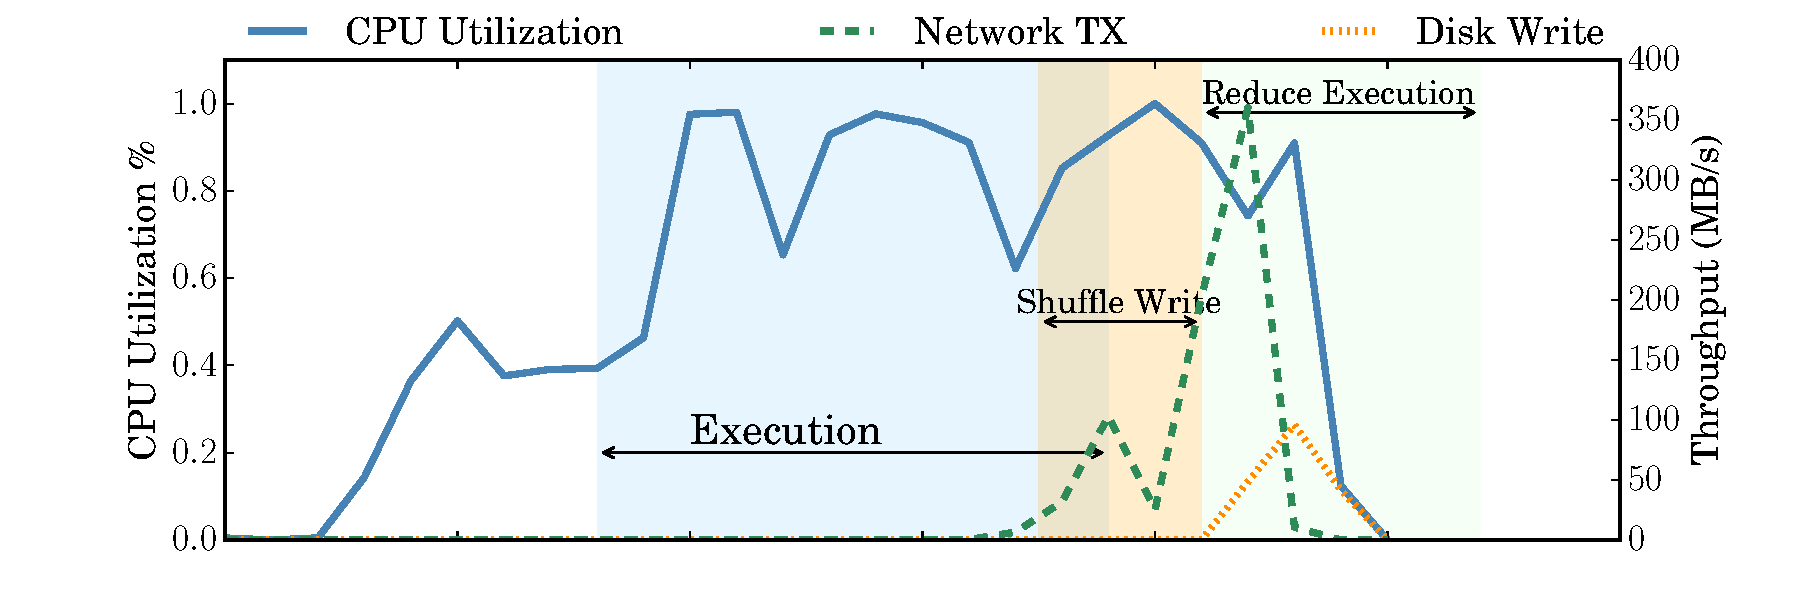
\includegraphics[width=\linewidth]{fig/scache_util}
		\caption{Spark With SCache}
		\label{fig:scache_util}
	\end{subfigure}
	\caption{CPU utilization and I/O throughput of a node during a Spark single shuffle application}
\end{figure*}

\subsubsection{Inefficient Persistent Storage Operation}
At first, both shuffle write and read are tightly coupled with task execution, which results in a blocking I/O operation. 
This blocking I/O operation along with synchronized shuffle read may introduce significant latency, especially in an I/O performance bounded cluster.
Besides, the legacy of storing shuffle data on disk is inefficient in modern clusters with large memory. 
Compared to input dataset, the size of shuffle data is relatively small. 
For example, the shuffle size of Spark Terasort is less than $25\%$ of input data. 
The data reported in \cite{makingsense} also show that the amount of data shuffled is less than the input data by as much as $10\%-20\%$. 
On the other hand, memory based distributed storage systems have been proposed \cite{memcached, tachyon, ramcloud} to move data back to memory, 
but most of the DAG frameworks still store shuffle data on disks (e.g., Spark \cite{apachespark}, Hadoop MapReduce, Dryad \cite{dryad}, etc).
We argue that the memory capacity is large enough to store the short-living shuffle data with cautious management.

\subsubsection{Multi-round Tasks Execution}\label{multi}
Both experience and DAG framework manuals(e.g., Hadoop\footnote{http://hadoop.apache.org/docs/current/hadoop-mapreduce-client/hadoop-mapreduce-client-core/MapReduceTutorial.html} and Spark\footnote{http://spark.apache.org/docs/1.6.2/configuration.html}) recommend that multi-round execution of each stage will benefit the performance of applications.
For a cluster with $n$ slots, the number of tasks should be $n \times k \; (k \geq 1)$. 
% For example, Hadoop MapReduce Tutorial\footnote{http://hadoop.apache.org/docs/current/hadoop-mapreduce-client/hadoop-mapreduce-client-core/MapReduceTutorial.html} suggests that \textit{10-100 maps} per-node and \textit{0.95 or 1.75 $\times$ number of nodes $\times$ number of maximum container reduces} per-node seem to be the right level of parallelism. 
% Spark configuration also recommends $2\text{-}3$ tasks per CPU core\footnote{http://spark.apache.org/docs/1.6.2/configuration.html} (i.e., $k = 2\text{-}3$).
Since the shuffle data becomes available as soon as the end of a task's execution, 
and the network is idle during the map stage ("Network TX" during map stage in Figure \ref{fig:util}), 
the property of multi-round tasks can be leveraged to hide the cost by starting shuffle data transfer at the end rounds of map tasks. 
% optimize the shuffle read operations if the destination host of the shuffle data can be predicted a priori. 
% There are at least two persistent storage operations for each shuffle data block. At first, Spark will write shuffle data to the persistent storage after map task execution (i.e. \textit{shuffle write} in Figure \ref{fig:util}). During the \textit{shuffle read}, Spark will read shuffle data from remote and local persistent storage, which is the second operation. The persistence of shuffle data was designed for fault tolerance. But we believe it is not necessary for today's cluster. Recall that shuffle data only exist in a short time scale. But the Mean Time To Failure (MTTF) for a server is counted in the scale of year \cite{tachyon}, which is exponential compared with the duration of a shuffle. In addition, the capacity of memory and network has been increasing rapidly in recent years. As a result, numbers of memory based distributed storage system have been proposed \cite{memcached, tachyon, ramcloud}. On the other hand, the size of shuffle data is relatively small. For example, shuffle size of Spark Terasort \cite{spark-tera} is less than 25\% of input data. The data reported in  \cite{makingsense} also shows that the amount of data shuffled is less than input data, by as much as 10\%-20\%. We argue that removing persistent storage and using memory to achieve shuffle fault tolerance is feasible and efficient.

% Based on these observations, most of the DAG frameworks share the execution paradigm as well as the expense of shuffle process. 
To mitigate the shuffle overhead, we propose an optimization that starts shuffle read ahead of reduce stage to overlap the I/O operations in multi-round map tasks, and uses memory to store the shuffle data. 
To achieve this optimization:
\begin{itemize}
	\item Shuffle process should be decoupled from task execution to achieve a fine granularity scheduling scheme.
	\item Reduce tasks should be pre-scheduled without launching to achieve shuffle data pre-fetching.
	\item Shuffle process should be taken over and managed outside DAG frameworks to achieve a cross-framework optimization.
\end{itemize}
% In the following section, we elaborate the methodologies to achieve three design goals.
